\documentclass[11pt,oneside]{book}
\usepackage{amsmath,amssymb,amsthm,graphicx,enumitem,float,wrapfig}
\usepackage{fullpage}
\usepackage[utf8]{inputenc}
\usepackage[english]{babel}
\usepackage{geometry}
\usepackage{marginnote}
\usepackage[inline]{asymptote}
\usepackage{subcaption}
\usepackage{microtype}
\usepackage{perpage} %the perpage package
\MakePerPage{footnote} %the perpage package command
\graphicspath{ {./image/} }
%\everymath{\displaystyle}

\catcode`\=13
\def{$\bowtie$}

\newtheorem{thm}{Theorem}[section]

\theoremstyle{remark}
\newtheorem* {rem}{Remark}

\theoremstyle{definition}
\newtheorem{prob}{Problem}[section]
\newtheorem{ex}{Example}[section]
\newtheorem*{soln}{Solution}
\newtheorem{defn}{Definition}[chapter]

\newcommand{\s}{\space}
\newcommand{\wrt}{with respect to\s}
\newcommand{\perdis}{perpendicular distance\s}
\newcommand{\cg}{center of gravity\s}
\newcommand{\xy}[1]{(x_{#1} ,y_#1)}
\newcommand{\oneton}[1]{{#1}_1 ,{#1}_2,\dots,{#1}_n}
\newcommand{\myvec}[1]{\overrightarrow{#1}}
\newcommand{\ddt}[1]{\frac{\,\mathrm{d}#1}{\,\mathrm{d}t}}
\newcommand{\dddt}[1]{\frac{\,\mathrm{d^2}#1}{\,\mathrm{d}t^2}}
\newcommand{\ddx}[1]{\frac{\,\mathrm{d}#1}{\,\mathrm{d}x}}
\newcommand{\dddx}[1]{\frac{\,\mathrm{d^2}#1}{\,\mathrm{d}x^2}}
\begin{document}
\title{Statics And Dynamics\linebreak(Class Note and Sir's PDF)}
\author{Mehedi Hasan}
\maketitle
\newpage
\pagenumbering{roman}
\tableofcontents
\newpage
\pagenumbering{arabic}
\part{Statics}
\chapter{Introduction}
\section{Definitions}
\textbf{Force:} Force is anything which changes or tend to change, the state of rest or uniform motion of a body.\\ \\
\textbf{Rest:} A body is said to be rest when it does not change its position \wrt\s it's surrounding objects.\\ \\
\textbf{Statics:} Statics is the science with treats the action of forces on bodies, the forces being so arranged that the bodies are at rest.\\ \\
\textbf{Dynamics:} The science which treats the action of forces on bodies in motion is called dynamics.\\ \\
\textbf{Particle:} A particle is a portion of matter which is indefinitely small in size.\\ \\
\textbf{Rigid Body:} A rigid body is a body whose parts always preserve an invariable position \wrt\s one another.\\ \\
\textbf{Equal Forces:} Two forces are said to be equal when if they act on a particle in opposite direction, the particle remains at rest.\\ \\
\textbf{Mass:} The mass of a body is the quantity of matter in the body.\\ \\
\textbf{Weight:} The force with which the earth attract any body to itself is called the weight of the body.\\ \\
\textbf{Tension:}If we tie one end of a string to any point of a body and pull at the other end of the string, we exert a force on that body, such a force exerted by means of string or rod is called tension.\\ \\
%TODO:need figure
\textbf{Equilibrium:} When two or more forces act upon a body and are so arranged that the body remains at rest, the forces are said to be in equilibrium.\\ \\
%TODO:need figure
\textbf{Resultant:} If two or more forces $P,Q,S\dots$ act upon a rigid body and it a single force $R$ can be found whose effect upon the body is the same as that of the forces $P,Q,S\dots$. This single force $R$ is called the resultant of the other forces and the forces $P,Q,S\dots$ are called the component of $R$.\\ \\
\textbf{Moments:} The moment (or torque) of a force about a turning point is the force multiplied by the perpendicular distance to the force from the turning point. Moments are measured in Newton meters(Nm). Mathematically \[\text{Moment}=F.d\]
\begin{ex}
  A $10 \,N$ force acts at a \perdis\s of $0.5m$ from the turning point. What is the moment of the force?
\end{ex}
\begin{soln}
  \begin{align*}
    M &= F\,.\,d \\
     &=10 \times 0.5  \\
     &=5 \,Nm
  \end{align*}
\end{soln}
\textbf{The principal of momentum:} When an object is in equilibrium, the sum of the anti-clockwise moments about a turning point
must be equal to the sum of the clockwise moments.\\ \\
\textbf{Couple:} Two forces of equal magnitudes and opposite direction whose line of action is not same is said to constitute a couple. A couple produces rotational effects in the body on which it acts and this rotational effect is measured by a physical quantity torque. Mathematically, $\text{Couple}= F.S$
\chapter{Reduction of a System of Coplanar Forces}
\section{Reduction of a System of Coplanar Forces}
\textbf{Statement: } A system of forces acting in one plane ar different point of a rigid body can be reduces to a single force $R$ through any arbitrary point and a couple, whose moment is equal to the sum of the moments of the given forces about this point.
\begin{proof}

  Let $O$ be any point in the plane. Through $O$ take any pair of rectangular axes $OX$ and $OY$ . Let the forces $P_1,P_2,P_3,\dots$ act at points $A_1(x_1,y_1),A_2(x_2,y_2),A_3(x_3,y_3),\dots$.\\
  \begin{figure}[H]
    \centering
    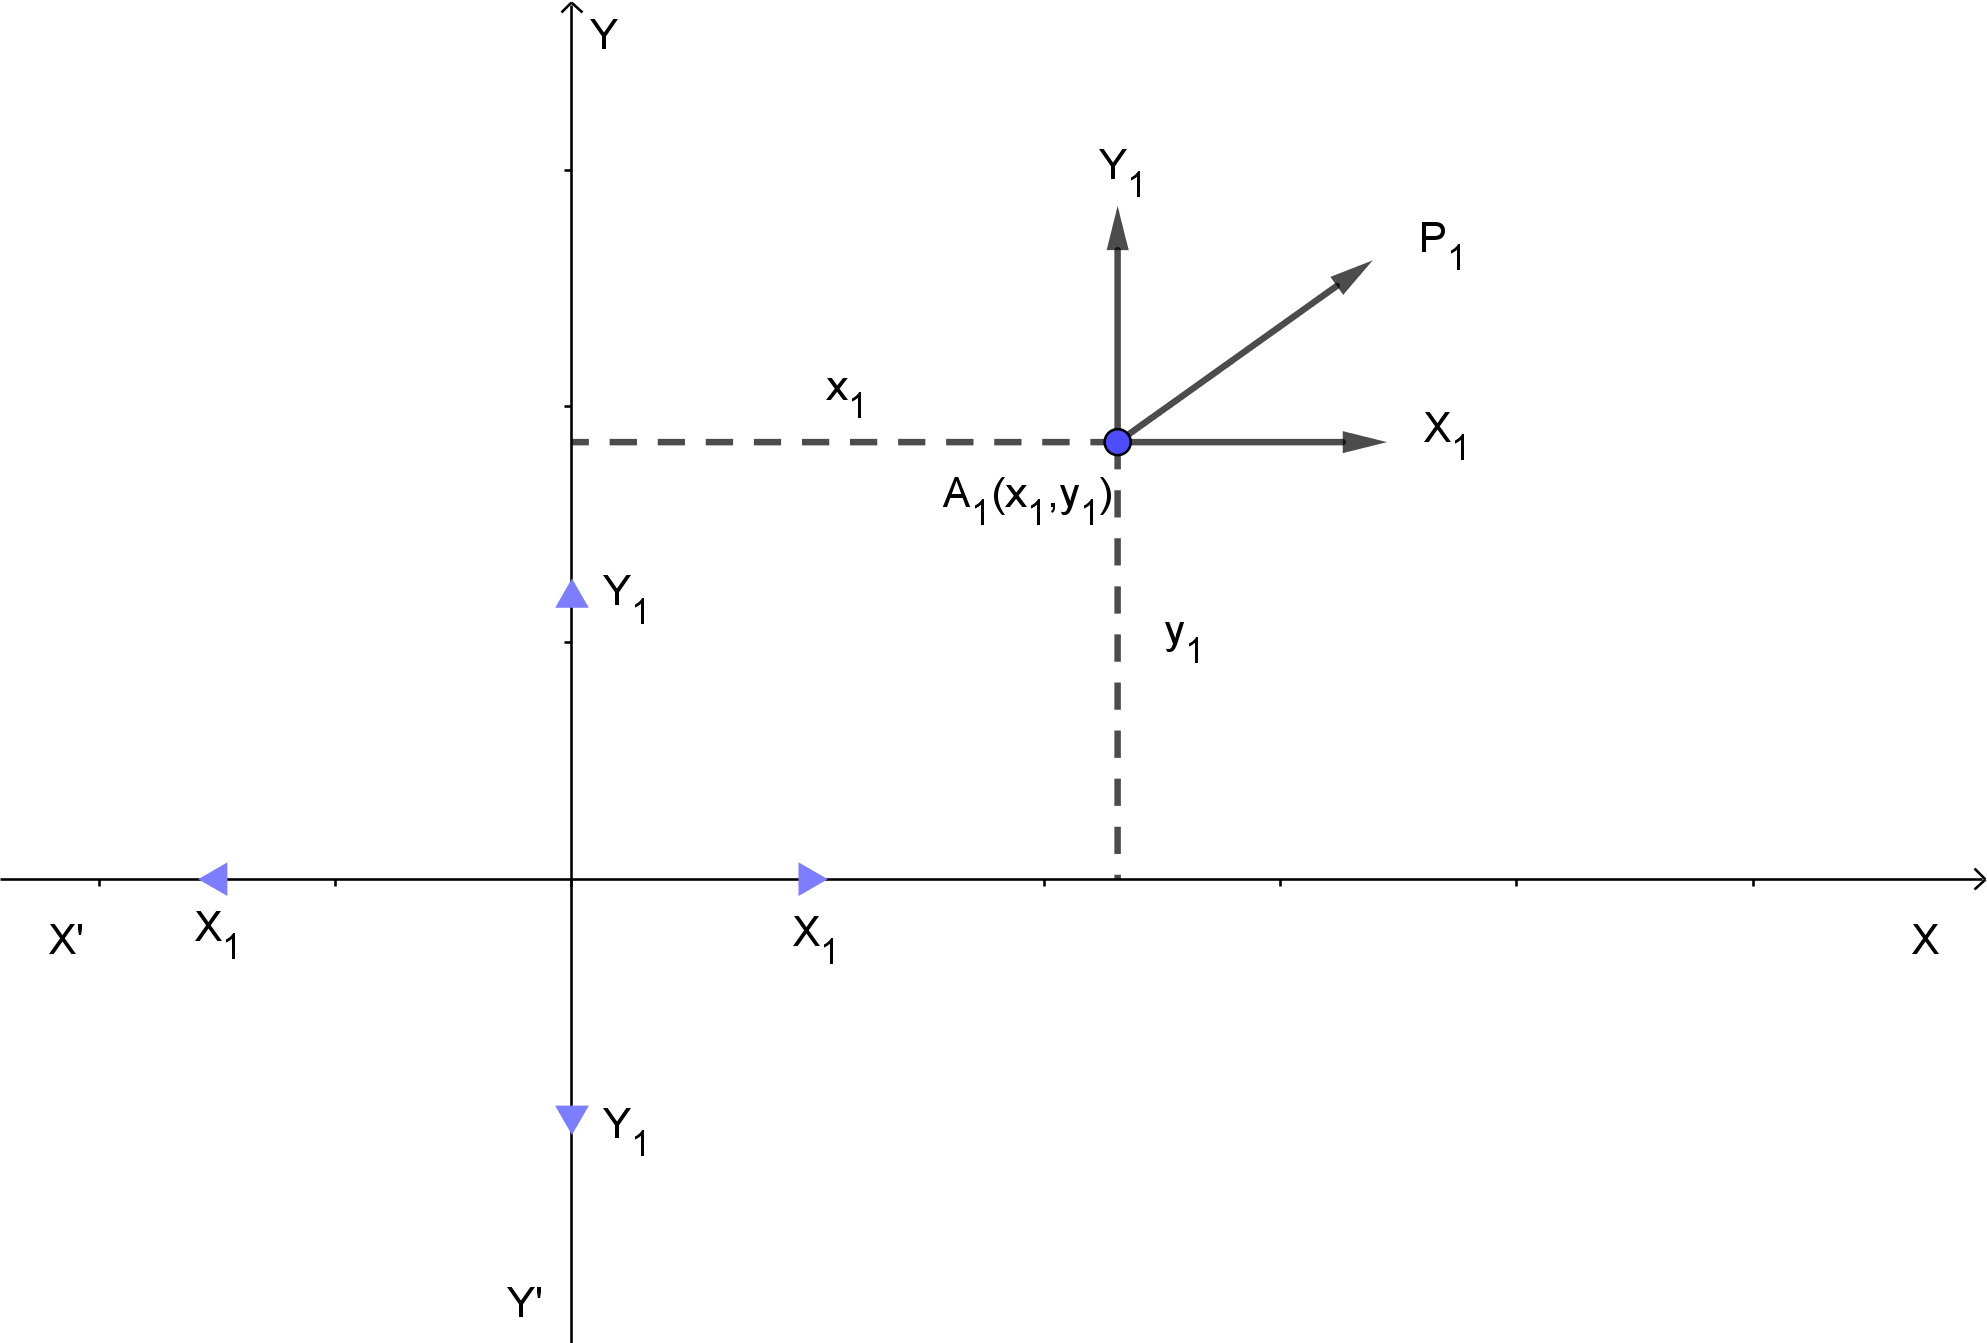
\includegraphics[height=7cm]{01}
    %\caption{}\label{}
  \end{figure}
  Let the resolved parts of these forces in direction parallel to the axes be $(X_1,Y_1),(X_2,Y_2),(X_3,Y_3),\dots$\\ \\
  At $O$ introduce forces $X_1$ and $X_1$ along $OX$ and $OX^\prime$ also $Y_1$ and $Y_1$ along $OY$ and $OY^\prime$ respectively. So that their actions $O$ are zero. i.e. the body remain unaffected.\\ \\
  Now the force $P_1$ at $A_1$ has component $X_1$ parallel to $OX$ and this component $X_1 \text{ at }O$ acts along $OX$. Another two equal forces $X_1$ at $A_1$ and $X_1$ at $O$ along $OX^\prime$ are equal and unlike parallel forces which form a couple of moment $-X_1 y_1$ and this couple has a tendency to rotate the body in a clockwise direction.\\ \\
  Similarly, the force $Y_1$ acting at $O$ along $OY^\prime$ and the force $Y_1$ as $A_1$ parallel to $OY$ form a couple of moment $x_1 Y_1$.\\ \\
  Hence the force $P_1$ at $A_1$ is equivalent to components $X_1,Y_1$ along $OX, OY$ and a couple $G_1=x_1Y_1-X_1y_1$, which is algebraic sum of the moments of two couples formed above.\\ \\
  Similarly the force $P_2$ at $A_2$ is equivalent to components $X_2$ along $OX$ and $Y_2$ along $OY$ and a couple of moment $G_2=x_2Y_2-X_2y_2$.\\ \\
  Resolving all other forces in similar way, if $R$ is the resultant of forces along $OX$ and $OY$ inclined at angle $\theta$ to $OX$.
  \\ \\
  $R \cos \theta=X=X_1+X_2+X_3+\dots=\sum X_i$\\
  $R \sin \theta=Y=Y_1+Y_2+Y_3+\dots=\sum Y_i$\\
  If $G$ represents the algebraic sum of the moments of the couple, then
  \[G=G_1+G_2+G_3+\dots=\sum(x_iY_i-X_iy_i)\]
  Thus,
  \begin{align*}
    R &= \sqrt{X^2+Y^2} \qquad\text{Where, $X=\sum X_i$ and $Y=\sum Y_i$}\\
    \theta & =\tan^{-1}\frac{Y}{X} \\
    G &= \sum(x_iY_i-X_iy_i)
  \end{align*}

\end{proof}

\section{Equation to the resultant of a system of forces in one plane}

We have studied that the system of coplanar forces can be reduced to a single force $R$ through $O$ inclined at an angle $\theta$ with $OX$ and a couple of moments $G$ about $O$.\\
\begin{figure}[h]
  \centering
  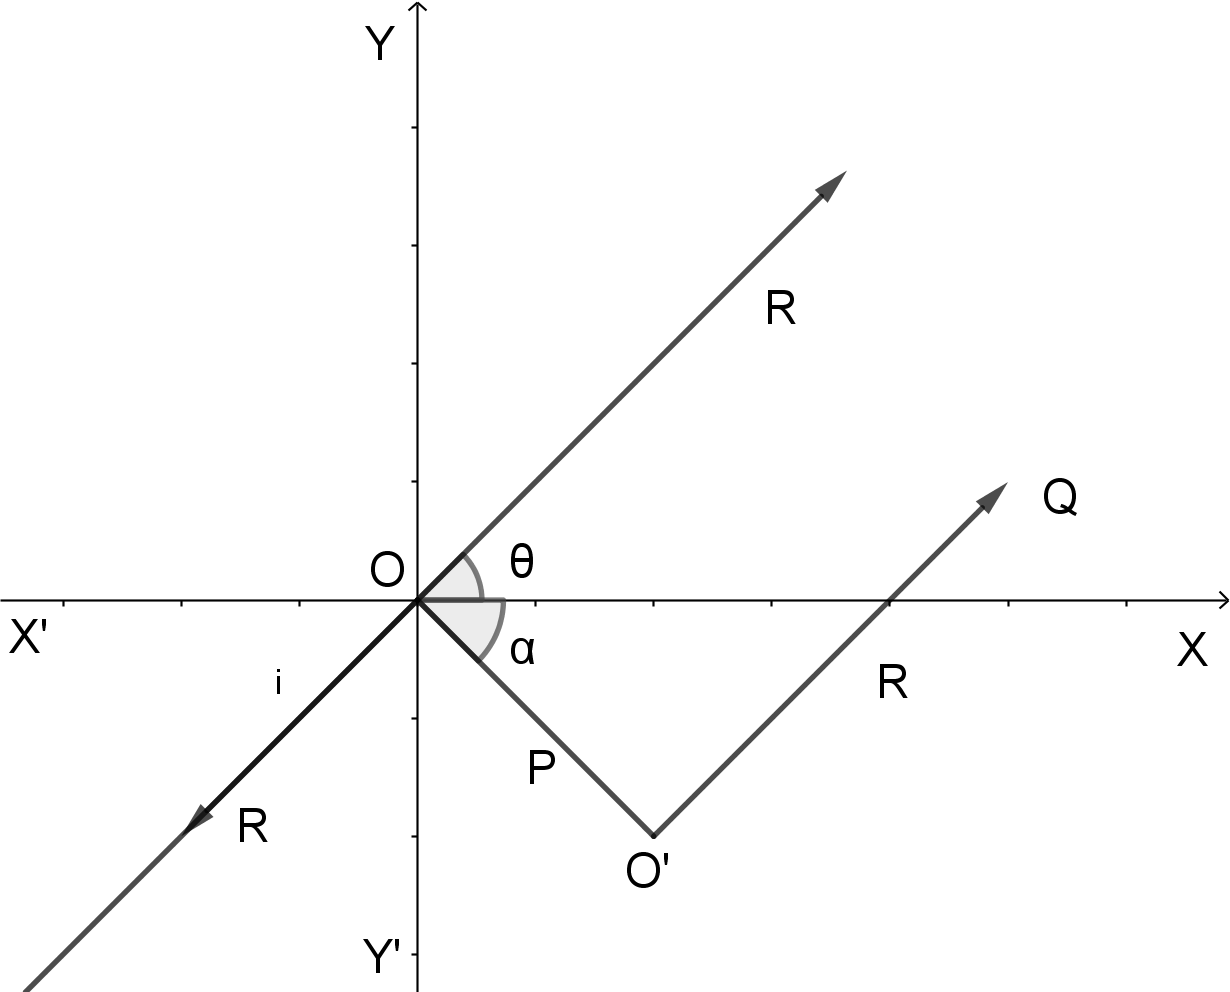
\includegraphics{02}
\end{figure}


Now replace the couple $G$ by two equal and unlike parallel forces one at $O$ opposite to the direction of $R$ and other at $O'$ perpendicular to $OO'$ so that,
\[
R.OO'\,=\,G\Rightarrow\, OO'\,=\frac{G}{R} \,\Rightarrow P=\frac{G}{R}
\]
Two forces at $O$ are equal and opposite and they cancel each other.\\

Another force $R$ at $O'$ along $O'Q$ where $OO'=P$ is left whose equation is to be determined.\\

Let $x\cos \alpha +y \sin \alpha=p$ be the equation of the line $OQ'$, where $OO'$ makes angle $\alpha$ with $OX$ and $OO'=p=\frac{G}{R}$.\\
Now, $\alpha=-\angle O'OX=-(\frac{\pi}{2}-\theta)$\\
Hence the equation of $O'Q$ is,
\begin{align*}
   & x\cos \left\{-\left(\frac{\pi}{2}\right)-\theta\right\}+y\sin  \left\{-\left(\frac{\pi}{2}\right)-\theta\right\}=\frac{G}{R}\\
  \Rightarrow\, & x\sin\theta-y\cos\theta=\frac{G}{R} \\
  \Rightarrow\, & x\,R\,\sin\theta-y\cos\theta=G \\
  \Rightarrow\, & xY-yX=G \qquad\qquad\left[\because X=R\cos\theta \text{ and }Y=R\sin\theta\right]\\
  \therefore\, & G-xY+yX=0
\end{align*}
\section{Condition of equilibrium of a system of coplanar forces}
We have,\[R=\sqrt{X^2+Y^2}\text{ and } G=\sum(x_iY_i-y_iX_i)\]
For equilibrium, \[R=0\quad\Rightarrow X=0,Y=0 \text{ and } G=0\]
The conditions of equilibrium can be stated as:
\begin{enumerate}[label=(\roman*)]
  \item The algebraic sum of the resolved parts of all the forces along $OX$ should be zero.
  \item The algebraic sum of the resolved parts of all the forces along $OY$ should be zero.
  \item The algebraic sum of the moments of all the forces about $O$ should be zero.
\end{enumerate}

Hence the necessary and sufficient conditions for equilibrium are $X=0,\,Y=0,\,G=0$.\\
These are known as the general conditions of equilibrium of forces.
\section{A static equilibrium}

A body is acted on by a system of coplanar forces, which keep it at rest. If all the forces are turned through the same angle about their points of application and if the equilibrium is not disturbed by such a rotation, then the equilibrium is said to be static.
\section{Theorems}
\begin{thm}
  If all the forces in a coplanar system are rotated about their angle in their own plane, their resultant passes through an fixed point in the body.
\end{thm}
\begin{proof}
  Let $P_1,P_2,P_3,\dots$ be the system of forces acting on the body at the points $\xy{1},\xy{2},\xy{3},\dots$ and make angle $\theta_1,\theta_2,\theta_3,\dots$ with $x$ axis. Let $X,Y$ be the components of the system along $OX, OY$ and $G$ be the moment of the forces about the origin.\\
  Now we have,
  \begin{equation}\label{eq:th1}
    \left.\begin{aligned}
            X &= \sum P_1 \,\cos\,\theta_1 \\
    Y &= \sum P_1 \,\sin\,\theta_1 \\
    G &= \sum P_1(x_1\,\sin \,\theta_1-y_1\,\cos\,\theta_1)
          \end{aligned}\quad
    \right\}
  \end{equation}
  The equation of the resultant is
  \begin{equation}\label{eq:th2}
    G-xY+Xy=0
  \end{equation}

  Let the forces be rotated through angle $\alpha$, about their points of applications, so that, $\theta_1,\theta_2,\dots$ becomes $\theta_1+\alpha,\theta_2+\alpha,\dots$. Let $X',Y'$ and $G'$ be the new system at the origin.\\
  Then,
  \begin{align*}
    X' & =\sum P_1\,\cos\,(\theta_1+\alpha) \\
     & =\sum (P_1\,\cos\,\theta_1\,\cos\,\alpha- P_1\,\sin\,\theta_1\,\sin\,\alpha)\\
     &= \sum (P_1\,\cos\,\theta_1)\,\cos\,\alpha-\sum( P_1\,\sin\,\theta_1\,)\sin\,\alpha \\
     &= X \,\cos \,\alpha-Y\,\sin\,\alpha\qquad\qquad\qquad\text{[by \ref{eq:th1}]}
  \end{align*}
  and,
  \begin{align*}
    Y' & =\sum P_1\,\sin\,(\theta_1+\alpha) \\
     & =\sum (P_1 \,\sin\,\theta_1\,\cos\,\alpha+P_1 \,\cos\,\theta_1\,\sin\,\alpha) \\
     & = \left(\sum P_1 \,\sin\,\theta_1\right)\,\cos\,\alpha+\left(\sum \,P_1 \,\cos\,\theta_1\right)\,\sin\,\alpha \\
     & =Y\,\cos \,\alpha+X\, \sin\,\alpha\qquad\qquad\qquad\text{[by \ref{eq:th1}]}
  \end{align*}
  and,
  \begin{align*}
    G' & =\sum \big\{P_1\,x_1\,\sin \,(\theta_1+\alpha)-P_1\,y_1\,\cos\,(\theta_1+\alpha)\big\} \\
     & =\cos \,\alpha\,\sum \,P_1(x_1\,\sin\,\theta_1-y_1\,\cos\,\theta_1)+\sin \,\alpha\,\sum \,P_1(x_1\,\cos\,\theta_1+y_1\,\sin\,\theta_1) \\
     & =G \,\cos\,\alpha+V\,\sin\,\alpha\qquad\qquad\qquad\text{[by \ref{eq:th1}]}
  \end{align*}
  Where, $V=\sum \,P_1(x_1\,\cos\,\theta_1+y_1\,\sin\,\theta_1)$ which is called \emph{viral of the system}.\\

  The equation of the new resultant of the system is
  \begin{align}\label{eq:th3}
     & G'-xY'+X'y=0 \notag \\
    \Rightarrow & \,G\cos\alpha+V\sin\alpha-x(Y\cos \alpha+X \sin\alpha)+y(X \cos \alpha-Y\sin\alpha)=0\quad\text{[Putting the value of $G',X',Y'$]} \notag\\
    \Rightarrow &\, \sin \alpha(xX+yY-V)+\cos\alpha(xY-yX-G)=0
  \end{align}
  \marginnote{Note:\\$x\sin\alpha+y\cos\alpha=0$ passes through the origin.} For all values of $\alpha$ \ref{eq:th3} passes through the intersection of $xX+yY-V=0$ and $xY-yX-G=0$.i.e. through the point
  \begin{equation}\label{eq:th4}
    \left(\frac{GY-VX}{X^2+Y^2},\frac{VY-GX}{X^2+Y^2}\right)
  \end{equation}
  Since the coordinates are independent of $\alpha$, hence it is a fixed point in the body. The point is called \emph{Astatic centre.}\\

  Suppose the forces are in equilibrium before displacement, then $X=0,\,Y=0$ and $G=0$.\\

  Hence after displacement, the system will be in equilibrium if,
  \begin{align*}
    X' & =X\cos\alpha-Y\sin\alpha=0 \\
    Y' & =Y\sin\alpha-x\cos\alpha=0 \\
    G' & =G\cos\alpha+V\sin\alpha=0
  \end{align*}
  The equilibrium will be static if $V=0$.\\
  Hence the equation for static equilibrium is $V=0$.\\

  From the above discussion, we came to the conclusion that if the original system of forces are in equilibrium and each is turned through an angle $\alpha$, they are equivalent to a couple whose moment is $V\sin\alpha$. Where $V$ is a constant independent of $\alpha$
\end{proof}
\newpage
\section{Problems}
\begin{prob}
  $ABCD$ is a square whose side is $2$ units in length. Forces $a,b,c,d$ act along the sides $AB,\,BC,\,CD,\,DA$ taken in order and $p\sqrt{2},\,q\sqrt{2}$ act along $AC$ and $DB$ respectively. Show that if $p+q=c-a\text{ and } p-q=d-b$, the forces are equivalent to a couple of moment $a+b+c+d$.
\end{prob}
\begin{soln}
  Resolve the forces along $AB \text{ and } AD$,
  \begin{figure}[h]
    \begin{subfigure}{0.5\textwidth}
    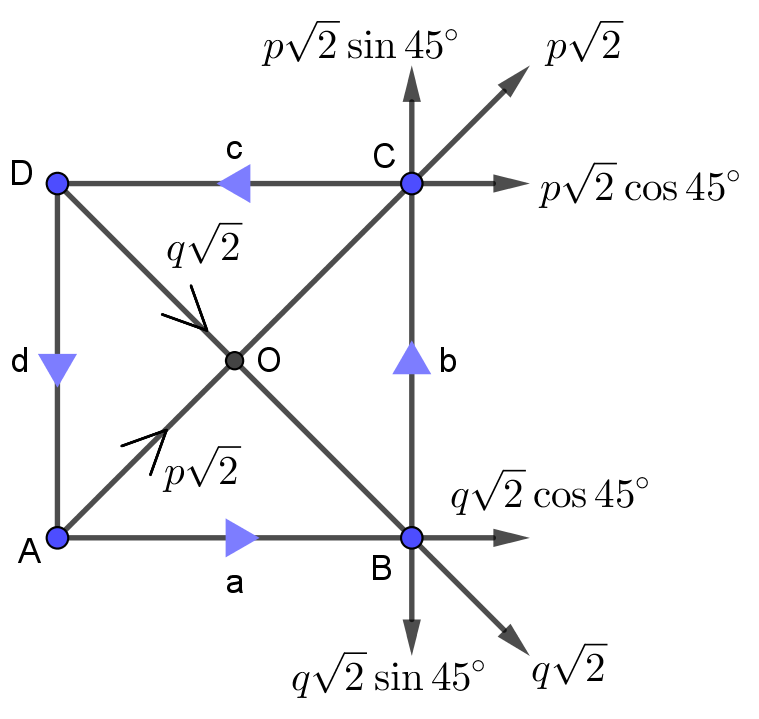
\includegraphics[scale=.3]{03}
    %\caption{}\label{}
    \end{subfigure}
    \begin{subfigure}{0.5\textwidth}
    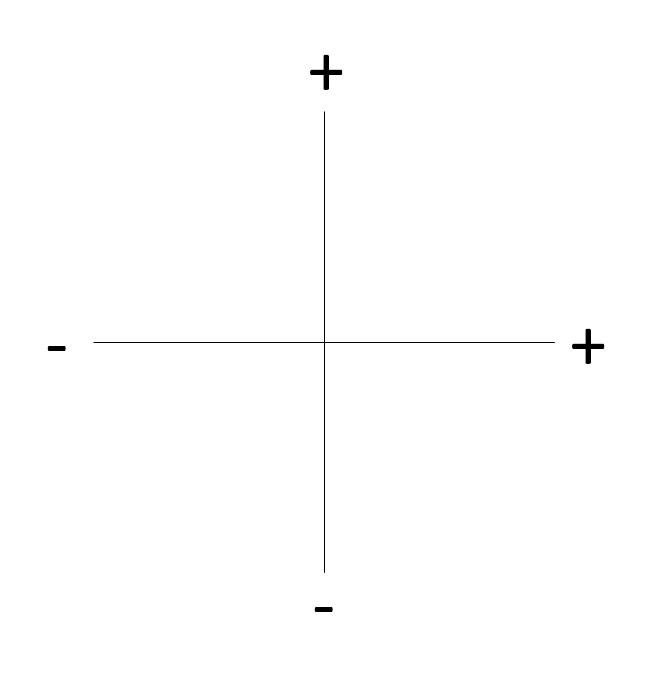
\includegraphics[scale=.3]{04}
    \end{subfigure}
  \end{figure}

  \begin{align*}
    X &= a-c+p\sqrt{2} \cos 45^\circ +  q\sqrt{2} \cos 45^\circ \\
     &= a-c+p+q \\
     &= 0\qquad[\therefore p+q=c-a] \\
    Y &= b-d+ p\sqrt{2} \sin 45^\circ -  q\sqrt{2} \sin 45^\circ\\
     &= b-d+p-q\\
     &= 0\qquad[\therefore p-q=d-b]
  \end{align*}
  Thus, there is no single resultant force.\\
  Take momentum about $A$,
  \begin{align*}
     &= b\,.\,2+c\,.\,2-q\sqrt{2}\,.\,\text{OA} \\
     & =2b+2c-q\sqrt{2}\,.\,2\cos 45^\circ \\
     & =2(b+c)-2q\qquad[\therefore p+q=c-a \text{ and }p-q=d-b] \\
     & =a+b+c+d
  \end{align*}
  %\reversemarginpar
  \marginnote{'+ve' in Anticlock wise and '-ve'in clock wise}
  \marginnote{Moment = Force$\times$perp. dist. If the force passes through the point then no moment.}[-5cm]
\end{soln}
\begin{prob}
  A rigid wire without weight in the form of the arc of a circle subtending an angle $\alpha$ at its centre and having two weights $P$ and $Q$ its extremties rests with its convexity downwards upon a horizontal plane. Show that if $\theta$ be the inclination to the vertical of the radius to the end at which $P$ is suspended then $\tan\theta=\frac{Q\sin\alpha}{P+Q\cos\alpha}$
\end{prob}
\begin{soln}
Let $ABC$ be the wire subtend an angle $\alpha=\angle AOB$ at
  the centre $O$. $OC$ is the vertical axis. $OA$ makes an angle $\theta$ with the vertical $OC$. $AM$ and $BN$ are the perpendicular drawn from $A$ and $B$ \wrt\s $OC$. Weights $P$ \& $Q$ are respectively acting at $A$ \& $B$.
  \begin{figure}[h!]
    \centering
    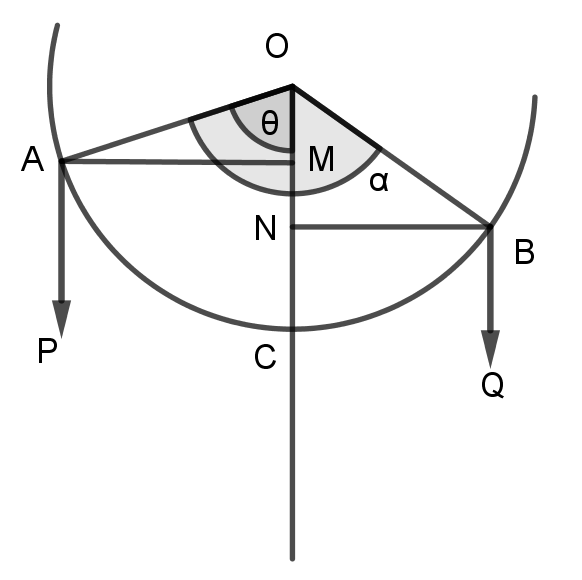
\includegraphics{05}
    \vspace{-40pt}
  \end{figure}


  Taking moment about $O$,
  \begin{align*}
     & P.AM-Q.BN=0 \\
    \Rightarrow\, &P.OA\sin\theta-Q.OB\sin(\alpha-\theta) =0 \\
    \Rightarrow\, & P\sin\theta=Q\sin\alpha\cos\theta-Q\cos\alpha\sin\theta\quad\text{[$\because OA=OB$]} \\
    \Rightarrow\, & P\tan\theta=Q\sin\alpha-Q\cos\alpha\tan\theta \\
    \Rightarrow\, & \tan\theta=\frac{Q\sin\alpha}{P+Q\cos\alpha}
  \end{align*}
\end{soln}
\newpage
\begin{prob}
  Forces $P,\,Q,\,R$ act along the sides $BC,\,CA,\,AB$ of the triangle $ABC$ and forces $P',\,Q',\,R'$ act along $OA,\,OB,\,OC$ where $O$ is the circumcenter in the sense indicated by the order of the letters. If the six forces are in equilibrium, show that \[
  \frac{PP'}{a}+\frac{QQ'}{b}+\frac{RR'}{c}=0\]
\end{prob}
\begin{soln}
  Let the area of $\Delta ABC=\Delta$\\
  \begin{figure}[h]
    \centering
    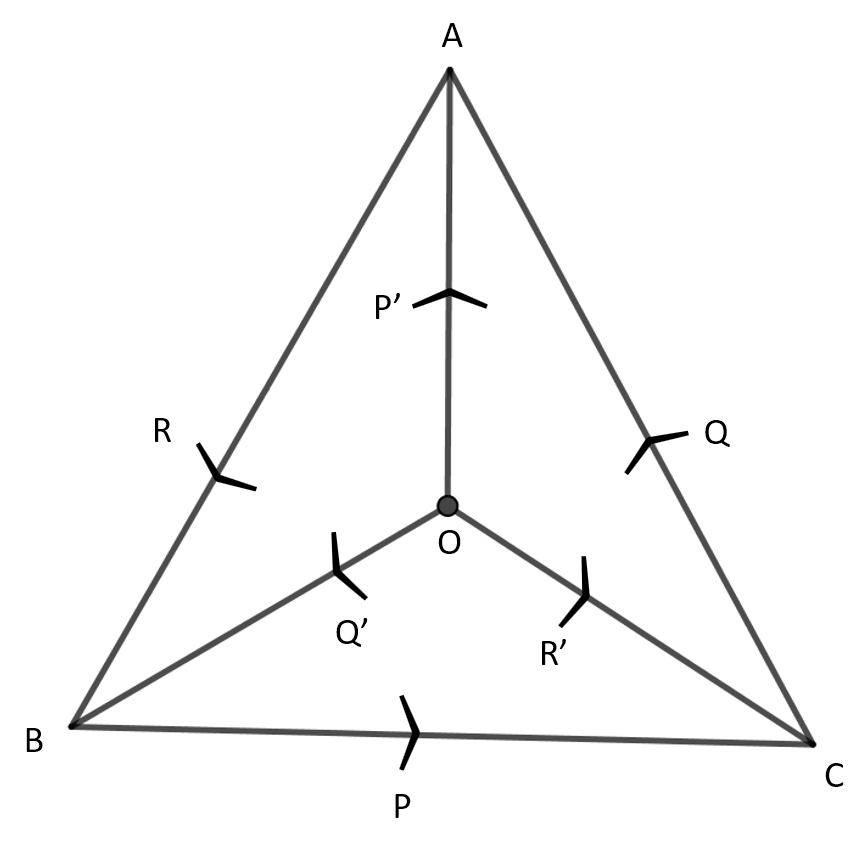
\includegraphics[scale=.5]{06}
  \end{figure}
  \\Consider $d_1=$ length of the perpendicular $A$ to $BC$, then,
  \begin{align*}
     & \Delta = \frac{1}{2}BC.d_1 \\
    \Rightarrow & d_1=\frac{2\Delta}{BC} \\
    \Rightarrow & d_1 = \frac{2\Delta}{a}
  \end{align*}
  Similarly, $d_2=\frac{2\Delta}{b},\,d_3=\frac{2\Delta}{c}$ where $d_2$ and $d_3$ are perpendicular from $B$ and $C$ to $ AC$ and $AB$ respectively.\\
  Again, length of perpendicular from $A$ to $CO$ is $P_1=\frac{2\Delta AOC}{OC}$\\
  Similarly, length of perpendicular from $A$ to $BO$ is $P_2=\frac{2\Delta BOA}{OB}$\\
  Similarly, length of perpendicular from $B$ to $OA$ and $B$ to $OC$ are\[P_3=\frac{2\Delta AOB}{OA}\quad\text{and }P_4=\frac{2\Delta BOC}{OC}\]
  and, length of perpendicular from $C$ to $OB$ and $C$ to $AO$ are\[P_5=\frac{2\Delta BOC}{OB}\quad\text{and }P_6=\frac{2\Delta AOC}{OA}\]
  Now, taking the moments of the forces about $A$,
  \begin{align*}
     & P.\frac{2\Delta}{a}+R'.P_1-Q'.P_2=0 \\
    \Rightarrow & P.\frac{2\Delta}{a}+R'.\frac{2\Delta AOC}{OC}-Q'.\frac{2\Delta BOA}{OB}=0
  \end{align*}
  Again, taking moment about $B$ and $C$ separately,
  \[
  Q.\frac{2\Delta}{b}+P'.\frac{2\Delta AOB}{OA}-R'\frac{2\Delta BOC }{OC}=0
  \]
  \[\text{and } R.\frac{2\Delta}{c}+Q'\frac{2\Delta BOC}{OB}-P.\frac{2\Delta AOC}{OA}=0\]
  Since, $OA=OB=OC=$ radius of the circumcircle. Multiply the equations by $P',Q',R'$ respectively and adding we get,
  \begin{align*}
     & PP'.\frac{2\Delta}{a}+QQ'\frac{2\Delta}{b}+RR'\frac{2\Delta}{c}=0 \\
    \Rightarrow & \frac{PP'}{a}+\frac{QQ'}{b}+\frac{RR'}{c}=0
  \end{align*}
\end{soln}
\newpage
\begin{prob}
  Three forces $P,Q,R$ act along the sides of a triangle formed by the lines $x+y=1,\,y-x=1$ and $y=2$. Find the equation of the line of the action of the resultant.
\end{prob}
\begin{soln}
The line of action of forces are shown in the figure.
\begin{figure}[h]
  \centering
  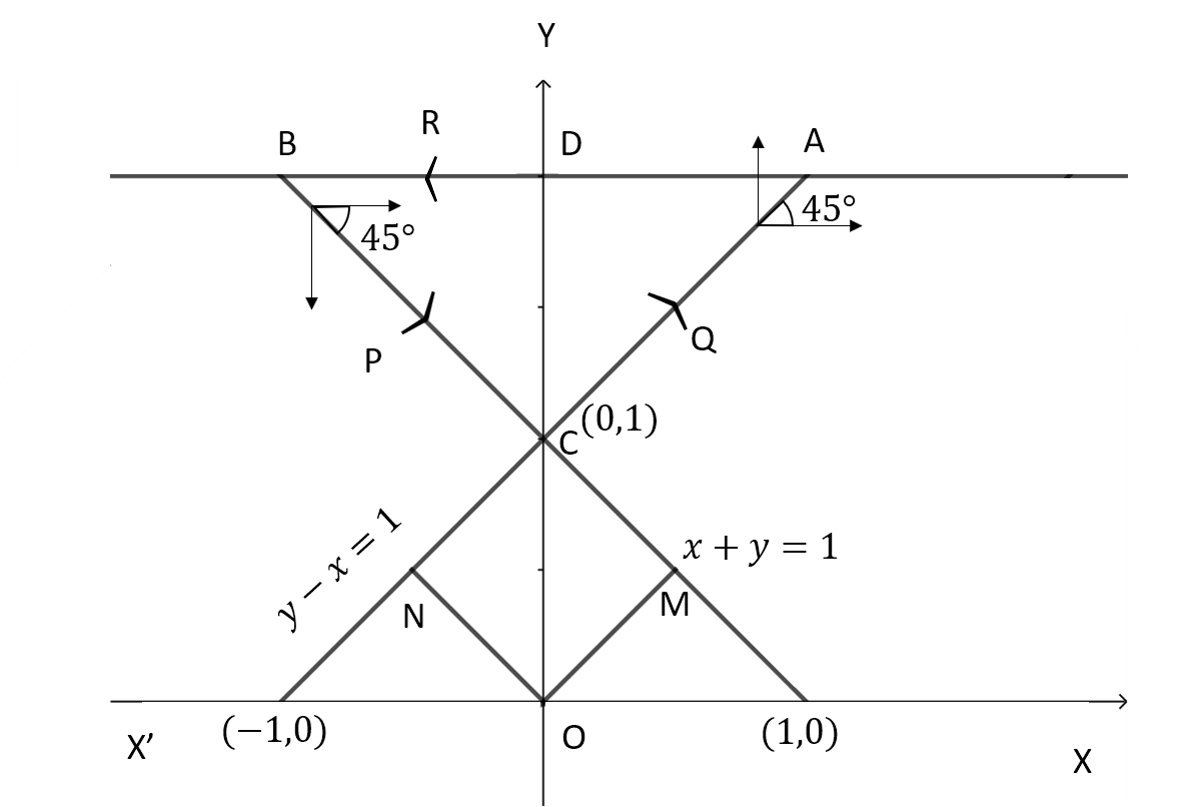
\includegraphics[scale=.5]{07}
  %\caption{}\label{}
\end{figure}
\\Resolve the forces along and perpendicular to $OX$
\begin{align*}
  X &= P.\cos45^\circ+Q\cos45^\circ+R\cos180^\circ \\
   &=(P+Q-R\sqrt{2})/\sqrt{2}  \\
  Y &= -P\sin45^\circ+Q\sin45^\circ+R\sin180^\circ \\
   &= -(P-Q)/\sqrt{2}
\end{align*}
Moments about $O$,
\begin{align*}
  G &= -P.OM-Q.ON+R.OD \\
   &= -P(1\sin45^\circ)-Q(1\sin45^\circ)+R(2) \\
   &=-(P+Q-2\sqrt{2}R)/\sqrt{2}
\end{align*}
The equation of the line action of the resultant is,
\begin{align*}
   & G+yX-xY=0 \\
  \Rightarrow & \frac{(-P-Q+2\sqrt{2}R)}{\sqrt{2}}+\frac{x(P-Q)}{\sqrt{2}}+\frac{y(P-Q-R\sqrt{2})}{\sqrt{2}}=0 \\
  \Rightarrow & P(x+y-1)+Q(y-x-1)-R(y-2)\sqrt{2}=0
\end{align*}
This is the required equation.
\end{soln}
\begin{prob}
  If six forces of relative magnitudes $1,2,3,4,5$ and $6$ act along the side of a regular hexagon taken in order. Show that the single equivalent force is of relative magnitude $6$ and that is acts along a line parallel to the force $5$ at a distance from the centre of the hexagon $3\frac{1}{2}$ times the distance of side from the centre.
\end{prob}
\begin{soln}
Let the horizontal and vertical through $O$ be taken as the axes of coordinates and $bc$ be the perpendicular distance of $O$ from each side.
\begin{figure}[h]
  \centering
  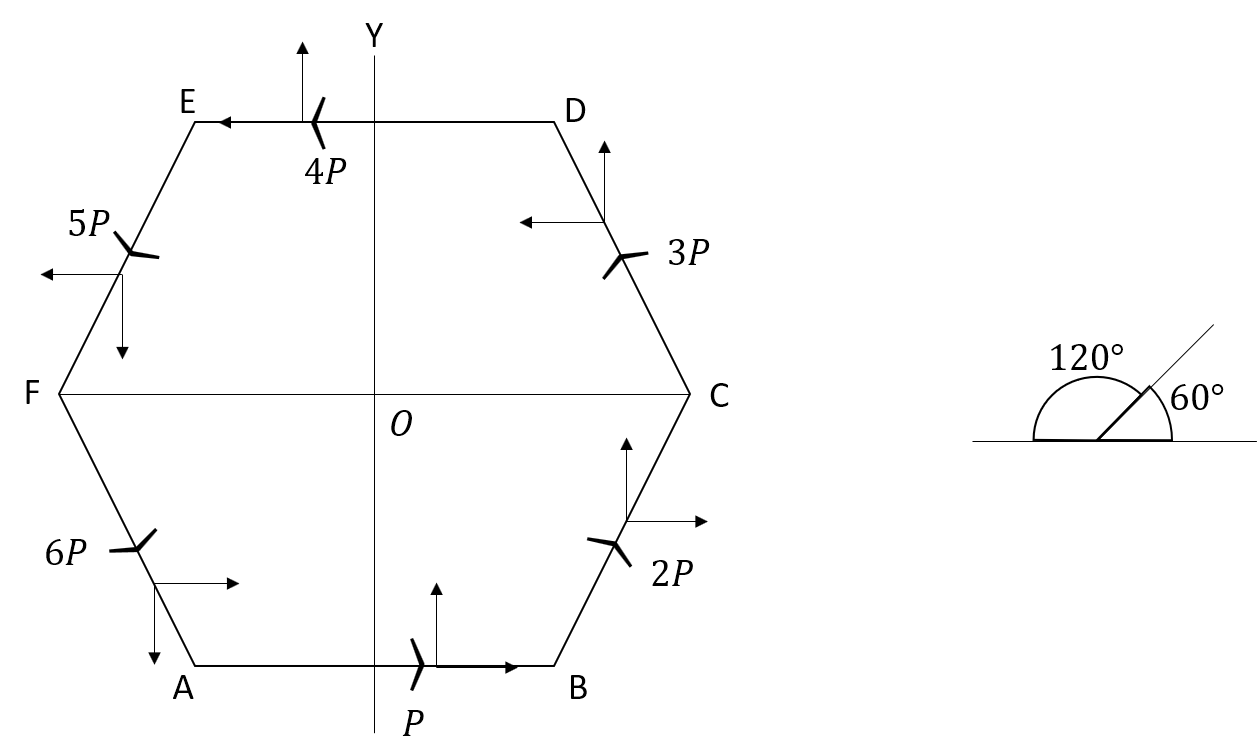
\includegraphics[scale=.5]{08}
  %\caption{}\label{}
\end{figure}
\\Resolve the forces along and perpendicular to $OC$
\begin{align*}
  X &=P+2P\cos60^\circ-3P\cos60^\circ -4P-5P\cos60^\circ+6P\cos60^\circ \\
   &=P+P-\frac{3P}{2} -4P-\frac{5P}{2}+3P \\
   &=-3P \\
  Y &=P\sin60^\circ+2P\sin60^\circ+3P\sin60^\circ+4P\sin180^\circ -5P\sin60^\circ-6P\sin60^\circ \\
   &=\sqrt{3}P+\frac{3\sqrt{3}P }{2}-\frac{5\sqrt{3}P}{2} -3\sqrt{3}P \\
   &= -3\sqrt{3}P
\end{align*}
Now,
\begin{align*}
  R &=\sqrt{X^2+Y^2}  \\
   &=\sqrt{9P^2+21P^2} \\
   &=6p
\end{align*}
and,
\begin{align*}
   & \tan\theta=\frac{Y}{X} \\
  \Rightarrow &\tan\theta=\frac{-3\sqrt{3}P}{-3P} \\
  \Rightarrow &\tan\theta=\sqrt{3} \\
  \Rightarrow &\tan\theta=\tan60^\circ \\
  \Rightarrow &\theta=60^\circ
\end{align*}
i.e., the resultant is parallel to the force $5P$.\\
Now the sum of the moments of the forces about $O$,
\begin{align*}
  G &= P.d+2P.d+3P.d+4P.d+5P.d+6P.d \\
   &= 21P.d
\end{align*}
Now, the equation of resultant is,
\begin{align*}
   &G+yX-xY=0 \\
  \Rightarrow &21Pd-3Py+3\sqrt{3}Px=0 \\
  \Rightarrow & \sqrt{3}x-y+7d=0
\end{align*}
Distance of the line acting of the resultant from $O(0,0)$ is
\[
P=\frac{0-0+7d}{\sqrt{(\sqrt{3})^2+1^2}}=\frac{7}{2}d=3\frac{1}{2}d
\]
\end{soln}
\textbf{H.W.} P.K Bhattacharjee, Ch-1: ex:1,2,3,4,6,8,9,11,15,17.
\chapter{Centre of Gravity}
\begin{defn}[center of Gravity]
  The center of gravity of a body or system of particles rigidly connected together is that point through which the line of action of the weight of the body always passes.
  \begin{figure}[h]
    \centering
    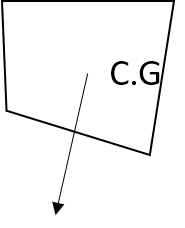
\includegraphics[scale=.5]{09}
  \end{figure}
\end{defn}
\section{General Formula for the determination of the center of gravity(2D)}
\subsection{For a scattered system of particle}
Let $w_1,w_2,\dots,w_n$ be the weights of a system of particles scattered on a plane situated at points $A_1,A_2,\dots,A_n$ respectively with coordinates $\xy{1},\xy{2},\dots,\xy{n}$. Let $(x',y')$ be the coordinates of their \cg $G$.

Now the weights of all particles are parallel to forces acting vertically downwards, hence their resultant force is a single force of magnitude $W=w_1+w_2+\dots+w_n$ acting at $G$ also vertically downwards.

Taking moment of forces about $OY$ axis then,
\begin{align*}
   &\, x'W=w_1x_1+w_2x_2+ \dots+w_nx_n\\
  \Rightarrow\, &\, x'W=\sum w_ix_i;\quad i=1,2,\dots,n\\
  \Rightarrow\, &\, x'=\frac{\sum w_ix_i}{W} \\
  \therefore\, &\, x'=\frac{\sum w_ix_i}{\sum w_i};\quad i=1,2,\dots,n
\end{align*}
Similarly by taking the moment of the forces about $OX$ axis, we have,
\begin{align*}
   &\, y'W=w_1y_1+w_2y_2+ \dots+w_ny_n\\
  \therefore\, &\, y'=\frac{\sum w_iy_i}{\sum w_i};\quad i=1,2,\dots,n
\end{align*}
\begin{rem}
For a scattered system of masses $\oneton{m}$ at $\oneton A$. Since the weights of the particles are proportional to their corresponding masses then $G(x',y')$ is,
\[
x'=\frac{\sum m_ix_i}{\sum m_i}\quad y'=\frac{\sum m_iy_i}{\sum m_i}
\]
\end{rem}

If we consider a continuous distribution of matter in the form of a rigid lamina of any shape, the coordinate \cg is ,
\[
x'=\frac{\sum x\delta w}{\delta w}\quad y'=\frac{\sum y\delta w}{\delta w}
\]

When $\delta w$ is the weight of a element of lamina with coordinates at $(x,y)$. If we subdivide the lamina into indefinitely large number of such ......., then $\delta w$ becomes an indefinitesimal and in the limit we have,
\begin{equation}\label{eq:cg1}
    \left.\begin{aligned}
            x'&= \frac{\int x \,\mathrm{d}w}{\int \,\mathrm{d}w},\quad y'=\frac{\int y \,\mathrm{d}w}{\int \,\mathrm{d}w} \\
    \text{or, }x'&= \frac{\int x \,\mathrm{d}m}{\int \,\mathrm{d}m},\quad y'=\frac{\int y \,\mathrm{d}m}{\int \,\mathrm{d}m}
          \end{aligned}\quad
    \right\}
  \end{equation}
  where the integration is such as to include the whole body.
  \newpage
\subsection{Center Of Gravity of an Arc}
\begin{wrapfigure}[10]{r}{6cm}
\vspace{-30pt}
\centering
 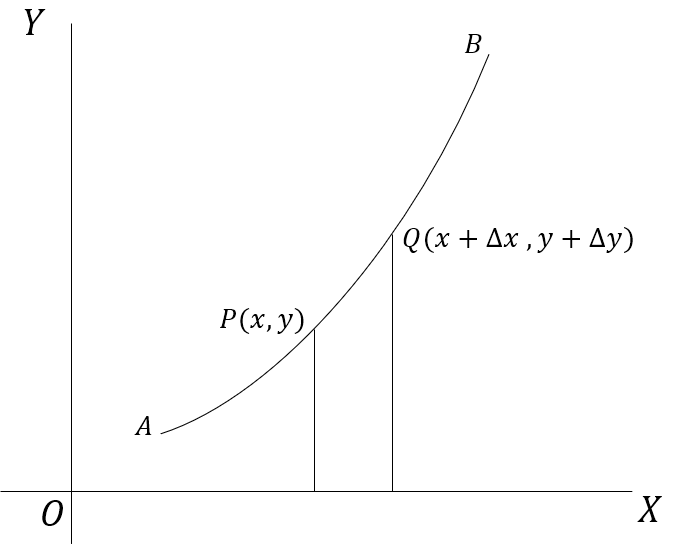
\includegraphics[scale=.5]{10}
\vspace{-10pt}
\end{wrapfigure}
Let, $AP=s$, $AQ=s+\Delta s$, $PQ=\Delta s$, and $\rho=$ density of the arc at $P$. Then $\,\mathrm{d}m=\rho\,\mathrm{d}s$.\\
$P(x,y),\, Q(x+\Delta x,y+\Delta y)$ and \cg $G(x',y')$ then,
\begin{equation}\label{eq:cg2}
  x'= \frac{\int x \rho\,\mathrm{d}s}{\int \rho\,\mathrm{d}s},\quad y'=\frac{\int y \rho\,\mathrm{d}s}{\int \rho\,\mathrm{d}s}
\end{equation}
The limit of integration extending from one end to the other of the arc considered.\\
If the density is uniform then,
\begin{equation}\label{eq:cg3}
    \left.\begin{aligned}
            x'&= \frac{\int x \,\mathrm{d}s}{\int \,\mathrm{d}s}=\frac{\int x \frac{\,\mathrm{d}s}{\,\mathrm{d}x}\,\mathrm{d}x}{\int\frac{\,\mathrm{d}s}{\,\mathrm{d}x}\,\mathrm{d}x}\\
    y'&= \frac{\int y \,\mathrm{d}s}{\int \,\mathrm{d}s}=\frac{\int y \frac{\,\mathrm{d}s}{\,\mathrm{d}y}\,\mathrm{d}y}{\int \frac{\,\mathrm{d}s}{\,\mathrm{d}y}\,\mathrm{d}y}
          \end{aligned}\quad
    \right\}
\end{equation}
Here, $\frac{\,\mathrm{d}s}{\,\mathrm{d}x}=\sqrt{1+\left(\frac{\,\mathrm{d}y}{\,\mathrm{d}x}\right)^2}$, $\frac{\,\mathrm{d}s}{\,\mathrm{d}y}=\sqrt{1+\left(\frac{\,\mathrm{d}x}{\,\mathrm{d}y}\right)^2}$\\

In polar coordinates, say, $r=f(\theta)$ \\then, $\Delta s=\sqrt{\Delta r^2+r^2(\Delta\theta)^2}$ and $x=r\cos\theta$, $ y=r\sin\theta$.\\
Then we have,
\begin{equation}\label{eq:cg4}
    \left.\begin{aligned}
            x'&= \frac{\int r\cos\theta.\rho \,\mathrm{d}s}{\int \,\mathrm{d}s}\\
    y'&= \frac{\int r \sin\theta.\rho \,\mathrm{d}s}{\int \,\mathrm{d}s}
          \end{aligned}\quad
    \right\}
\end{equation}
\subsection{Center of Gravity of a Plane}
If $\,\mathrm{d}A$ be an elementary area whose \cg is at $P(x,y)$ and $\rho$ is the mass per unit area at $P_1$ then,
\[
x'=\frac{\int \rho x\,\mathrm{d}A}{\int \rho \,\mathrm{d}A},\quad y'=\frac{\int \rho y\,\mathrm{d}A}{\int \rho \,\mathrm{d}A}
\]
In cartesian coordinate, $\,\mathrm{d}A=\,\mathrm{d}x\,\mathrm{d}y$, then,
\begin{equation}\label{eq:cg5}
  x'=\frac{\iint \rho x\,\mathrm{d}x\,\mathrm{d}y}{\iint \rho \,\mathrm{d}x\,\mathrm{d}y},\quad y'=\frac{\iint \rho y\,\mathrm{d}x\,\mathrm{d}y}{\iint \rho \,\mathrm{d}x\,\mathrm{d}y}
\end{equation}

In polar coordinate, \begin{equation*}
                       \begin{aligned}
                       \,\mathrm{d}A&=r\,\mathrm{d}r\,\mathrm{d}\theta\\
                       x&=r\cos\theta\\
                       y&=r\sin\theta
                       \end{aligned}
                     \end{equation*}
then,
\begin{equation}\label{eq:cg6}
    \left.\begin{aligned}
            x'&= \frac{\iint \rho \,r\cos\theta r\,\mathrm{d}r\,\mathrm{d}\theta}{\iint \rho r\,\mathrm{d}r\,\mathrm{d}\theta}=\frac{\iint \rho \, r^2 \,\cos\theta \,\mathrm{d}r\,\mathrm{d}\theta }{\iint \rho r\,\mathrm{d}r\,\mathrm{d}\theta}\\
    y'&= \frac{\iint \rho \,r\sin\theta r\,\mathrm{d}r\,\mathrm{d}\theta}{\iint \rho r\,\mathrm{d}r\,\mathrm{d}\theta}=\frac{\iint \rho \, r^2 \,\sin\theta \,\mathrm{d}r\,\mathrm{d}\theta }{\iint \rho r\,\mathrm{d}r\,\mathrm{d}\theta}
          \end{aligned}\quad
    \right\}
\end{equation}
\subsection{Center of Gravity of area bounded by the curve $ y=f(x)$, $x-$axis and coordinates $x=a$ and $x=b$, when density is uniform}
\begin{figure}[h]
  \centering
  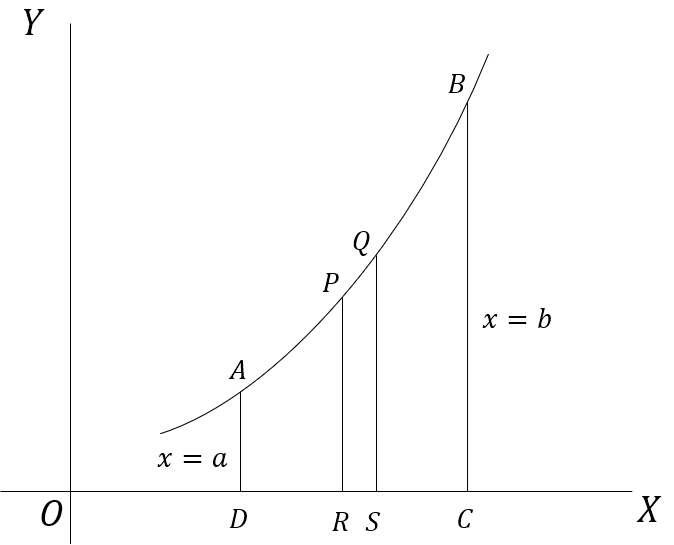
\includegraphics[scale=.5]{11}
\end{figure}
\begin{equation}\label{eq:cg7}
  x'=\frac{\int_{a}^{b}xy\,\mathrm{d}x}{\int_{a}^{b}y\,\mathrm{d}x},\quad y'=\frac{1}{2}\frac{\int_{a}^{b}y^2\,\mathrm{d}x}{\int_{a}^{b}y\,\mathrm{d}x}
\end{equation}
\begin{rem}
If area is symmetric \wrt $x$-axis, the \cg is at $(x',0)$, and for symmetric about $y-$axis \cg is at $(0,y')$.
\end{rem}
\newpage
\subsection{Center of Gravity of the area bounded between the curve $r=f(\theta)$ and two radii vector $\theta=\alpha,\,\theta=\beta,\,\rho$ is the density of the uniform curve}
\chapter{Moments of Inertia}
\part{Dynamics}
\chapter{Kinematics In Two Dimensions}
\section{Displacement} When a point changes its position and occupies different positions at different times relative to an object which we consider to be fixed, then the point is said to be in motion and is displaced. The curve drawn through the successive positions of the particle is called its \emph{path.}
\begin{defn}[Displacement]
  Let us take a particle at a point $P$ and later on it shifts to another point $Q$. We say that $P$ is displaced from $P$ to $Q$ and $PQ$ is called displacement.
\end{defn}
We should note here that $PQ$ has a magnitude as well as direction $P\rightarrow Q$ and hence it is a vector quantity. The particle in reaching $Q$ may travel along a straight line or a curved path. We shall first confine our attention to displacement in a straight line.

\section{Velocity} Consider a point $O$ taken to be fixed and relative to which we shall consider the motion of a particle which moves along the straight line $OX$. The position $P$ of the particle at any instant is the defined by $\myvec{OP}$. At any subsequent instant let it be at $Q$; then $PQ$ is the displacement during that interval of time. If the time required to move a distance $PQ$ along the line be $t$ then $\frac{PQ}{t}$ measures the average velocity of the particle during the interval $t$. We thus have \emph{average velocity = $\frac{\text{displacement}}{\text{time}}$} or we may define velocity as the rate of displacement. If the particle moves at a uniform rate (i.e. it covers equal distance in equal times) the velocity is uniform or it is said to be moving with uniform velocity. Here again we should note that it is a vector quantity because the rate of displacement in a given direction is termed as velocity in that direction.\\

Two velocities may have same magnitude but different directions and hence they will not be called equal. Whenever we may say that a velocity is changing it may mean that there is only change in its magnitude or only in its direction or change in both.\\

Let again the particle be at $P$ at a distance $x$ from the fixed point $O$ and let it be displaced to a point $P'$ such that $PP'=\delta x$ during an interval of time $\delta t$ when $ \delta t$ is small, then $\delta x/\delta t$ is the average velocity during this interval. The particle may not be moving at a uniform rate during that interval and hence we have called it average velocity. As we decrease the interval $\delta t$ and make it smaller and smaller, velocity of the particle during the interval differs from its velocity at $P$ by a smaller and smaller amount. Ultimately if we think that $\delta t \rightarrow0$ so also $\delta x$ (because $\delta x$ depends on $\delta t$ whatever the velocity may be), the velocity during the infinitesimal interval $\delta t$ will be the same as that of the particle when at $P$.\\

Hence $v=\lim_{\delta t \rightarrow0} \frac{\delta x}{\delta t}=\frac{\,\mathrm{d}x}{\,\mathrm{d}t}$ along x increasing.\footnote{Usually differential coefficient of variables with regard to time are denoted by putting dots above them, e.g. $\frac{\,\mathrm{d}x}{\,\mathrm{d}t}=\dot{x},\frac{\,\mathrm{d}u}{\,\mathrm{d}t}=\dot{u},\frac{\,\mathrm{d^2}x}{\,\mathrm{d}t^2}=\ddot{x}$ etc.}\\
Speed is a scaler quantity or it is only the magnitude of velocity while velocity has a direction too.

\section{Acceleration} When the velocity is not uniform it may increase or decrease.
\begin{defn}[Acceleration]
  The rate of change of velocity os defined as acceleration.
\end{defn}
If $v$ be the velocity of the particle at certain instant $t$ and $v+\delta v$ be its velocity after small subsequent interval $\delta t$ i.e. at time $t+\delta t$, then the acetylation $f$ is given by
\begin{align*}
  f &= \lim_{\delta t \rightarrow0}\frac{\text{change in velocity duting the small interval $\delta t$}}{\delta t} \\
   &=  \lim_{\delta t \rightarrow0}\frac{(v+\delta v)-v}{\delta t} \\
   &=  \lim_{\delta t \rightarrow0}\frac{\delta v}{\delta t} \\
   &= \ddt v
\end{align*}
Thus acceleration is given by $\,\mathrm{d}v/\,\mathrm{d}t$; but we have, $v=\ddt x$;
\[
\therefore f=\ddt v=\frac{\,\mathrm{d}}{\,\mathrm{d}t}\left(\ddt x\right)=\dddt x=\ddot{x}
\]
Again
\[
f=\ddt v =\ddx v \cdot \ddt x = v \ddx v
\]
\section{Motion in a Plane Curve}
\subsection{Cartesian System}
 \begin{wrapfigure}[12]{r}{6cm}
\vspace{-30pt}
\centering
 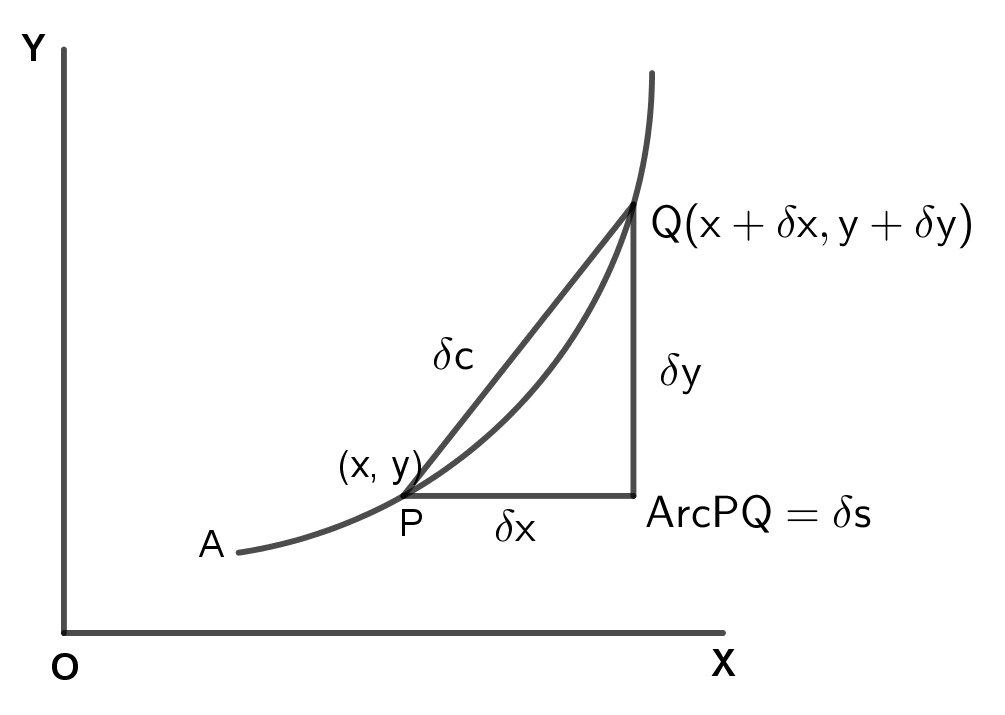
\includegraphics[scale=1]{d1}
\vspace{-10pt}
\end{wrapfigure}
Taking the first case, let $O$ be the origin (a fixed point), $ OX$ and $OY$ be two axes perpendicular to one another.Let the particle be at a point $P\,(x,y)$ at a given instant. Let it then move to a point $Q\,(x+\delta x,y+\delta y)$ during a subsequent interval $\delta t$ or at time $t+\delta t$. This suggests that during this interval the particle has gone to $Q$ along a curved path and the displacements in the $x$ and $y$ directions respectively are $\delta x$ and $\delta y$.

Let the path of the particle be $APQ$ where $A$ be a point from where we measure the distance along the arc. During the interval $\delta t$ the displacement of the particle is given by the chord $PQ$ and hence the velocity is given by $\frac{\text{chord }PQ}{\delta t}$ provided $\delta t \rightarrow0$.
\[\therefore\text{ Velocity at $P$ at time $t$}=\lim_{\delta t \rightarrow0}\frac{\text{chord }PQ}{\delta t}=\lim_{\delta t \rightarrow0}\frac{\text{chord }PQ}{\delta s}\cdot\frac{\delta s}{\delta t}\]
Where $\delta s$ represents the arcual distance $PQ$ along the curved path, $s$ being measured from $A$. As $\delta t \rightarrow0$ we have $\delta s$ also small and in limit chord $ PQ$ and $\delta s$ become equal.
\[
\therefore\text{ Velocity }=\lim_{\delta t \rightarrow0}\frac{\text{chord }PQ}{\delta s}\cdot\frac{\delta s}{\delta t}=1\times\frac{\delta s}{\delta t}=\ddt s
\]
As $Q$ approaches $P$ the chord $PQ$ becomes the tangent to the curve at $P$ and also in the direction in which $s$ is increasing.\\
Hence velocity at $P$ is given by $\ddt s$ and its direction is along the tangent to the curve at $P$ int the sense of $s$ increasing.\\
As given above the displacement $\myvec{PQ}$ is made up of two components, one $\delta x$ along the direction of $x$-axis and the other $\delta y$ along the direction of $y$-axis.\\ The component of velocity along the $x$-axis,
\[
\lim_{\delta t \rightarrow0}\frac{\text{displacement in direction of $x$-axis}}{\delta t}=\lim_{\delta t \rightarrow0}\frac{\delta x}{\delta t}=\ddt x=\dot{x}
\]
Similarly the component of velocity along the $y$-axis$=\ddt y=\dot{y}$\\

Hence if the co-ordinates of a particle be $(x,\,y)$ then components of its velocity parallel to $x$ and $y$ axes are given by $\ddt x$ and $\ddt y$ respectively.\\
Since the two components of velocity are along perpendicular direction, therefore resultant velocity $v$ is given by,
\[v^2=\left(\ddt x\right)^2+\left(\ddt y\right)^2\text{ or }v=\sqrt{\dot{x}^2+\dot{y}^2}\]
and the direction is given by $\tan \psi =\frac{\dot{y}}{\dot{x}}$ where $\psi$ is the angle which the direction of resultant velocity makes with $x$-axis.
\section{Components of Acceleration of a Particle in a Plane}
Let $u$ and $v$ be the components of velocity of the particle parallel to the axes when the particle is at $P$ at time $t$ and $u+\delta u,\,v+\delta v$ be those at time $t+\delta t$ when the particle is at $Q$. The changes in velocity during the interval $\delta t$ in the direction of axes are then $\delta u$ and $\delta v$.\\
Hence acceleration along $x-$axis,
\[
\lim_{\delta t \rightarrow0}\frac{\text{change of velocity in direction of $x$-axis}}{\delta t}=\lim_{\delta t \rightarrow0}\frac{\delta u}{\delta t}=\frac{\,\mathrm{d}}{\,\mathrm{d}t}\left(\ddt x\right)=\dddt x=\ddot{x} \text{ or } u\ddx u
\]
Similarly component of acceleration along the $y-$ axis
\[
\ddt v=\frac{\,\mathrm{d}}{\,\mathrm{d}t}\left(\ddt y\right)=\dddt y=\ddot{y}  \text{ or } v\frac{\,\mathrm{d}v}{\,\mathrm{d}y}
\]
and the resultant acceleration $f=\sqrt{\ddot{x}^2+\ddot{y}^2}$\\
and the resultant will make an angle $\tan^{-1} \frac{\ddot{y}}{\ddot{x}}$, with the $x-$axis.

\section{Problems}
\begin{prob}
  A particle moves along a straight line such that its displacement $x$ from a fixed point on the line at time $t$, is given by $x=t^3-9t^2+24t+6$. determine the following.
  \begin{enumerate}[label=(\roman*)]
    \item The instant when the acceleration becomes zero.
    \item The position of the particle at that instant.
    \item The velocity of the particle at that instant.
  \end{enumerate}
\end{prob}
\begin{soln}
Given,\[x=t^3-9t^2+24t+6\]
Now,
\begin{align*}
  \ddt{x} &= 3t^2-18t+24 \\
  \dddt{x} &= 6t-18
\end{align*}
so,
\begin{align*}
   &\,6t-18= 0 \\
  \Rightarrow &\,t= 3
\end{align*}
$\therefore$ the acceleration becomes zero when $t$ is $3$.\\
At $t=3$ the position of the particle is,
\begin{align*}
   &x= (3)^3-9(3)^2+24(3)+6 \\
  \Rightarrow & x=24
\end{align*}
At $t=3$ the velocity of the particle is,
\begin{align*}
   & v= 3(3)^2-18(3)+24 \\
  \Rightarrow & v=-3
\end{align*}
\end{soln}
\end{document} 